Dans cette section, l'objectif est de proposer une formulation de la condition en limite en $x=0$ du problème présenté
en figure~\ref{fig:rflx:propa_1D} qui n'impose pas de rajouter une ligne au système d'équations de la FEM.

\begin{figure}[!ht]
	\centering
	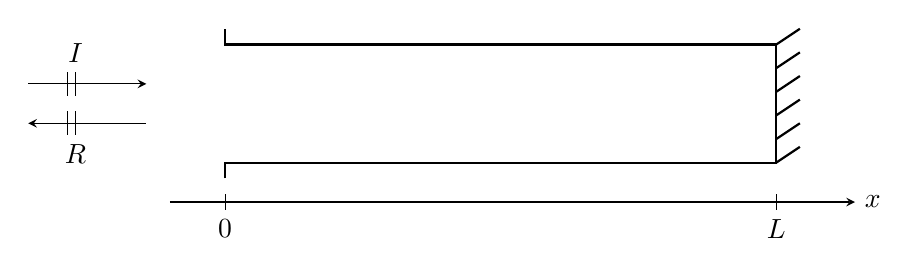
\begin{tikzpicture}[>=stealth]

	% waveguide
	\draw[thick] (0,.3) -- (0,.5) -- (7,.5) -- (7,2) -- (0,2) -- (0,2.2);
	\foreach \i in {0,...,5}{
		\draw[thick] (7,\i*0.3+0.5) -- ++(.3,.2);
	}
	
	% x axis
	\draw[->] (-.7,0) -- (8,0) node[right] {$x$};
	\draw (0,.1) -- ++(0,-.2) node[below] {$0$};
	\draw (7,.1) -- ++(0,-.2) node[below] {$L$};

	% waves
	% R
	\draw[<-] (-2.5,1) -- ++(1.5,0);
	\draw (-2,1.15) -- ++(0,-.3);
	\draw (-1.9,1.15) -- ++(0,-.3) node[below] {$R$};

	% I
	\draw[->] (-2.5,1.5) -- ++(1.5,0);
	\draw (-2,1.65) -- ++(0,-.3);
	\draw (-1.9,1.65) node[above] {$I$} -- ++(0,-.3);

\end{tikzpicture}


	\caption{\label{fig:rflx:propa_1D}Schéma du problème de propagation dans une cavité acoustique 1D de longueur L.}
\end{figure}

\section{Retour sur les conditions aux limites en MEF}

Pour ce problème et en utilisant le formalisme des éléments finis, le système à résoudre avant l'application de la
condition limite en $x=0$ mais après celle de la condition en $x=L$ est tel que présenté en~\eqref{FEM1D:post_BCL} :

\begin{equation}
\left[- \uul{K} + k^2\uul{M}\right]\GP = \begin{Bmatrix} \nabla p\bigg|_0\\0\\\vdots\\0\end{Bmatrix} \label{rflx:FEM}
\end{equation}


\subsection{Utilisation de la formulation de Galerkin}

Sous le formalisme de la méthode de Galerkin, il vient :

\begin{equation}
	j\omega\begin{Bmatrix}v\\p\end{Bmatrix} = 
		\underbrace{\begin{bmatrix}0 & \nicefrac{1}{\rho}\\\rho c^2 & 0\end{bmatrix}}_{\uul{F}}
		\begin{Bmatrix}v\\p\end{Bmatrix} \Leftrightarrow j\omega\ul{u} + \uul{P\Lambda Q}\ul{u} = 0
		\label{rflx:begin_dgm}
\end{equation}

Où $\uul{P\Lambda Q}$ est une diagonalisation de $\uul{F}$ telle que :

\[
\uul{P} = \begin{bmatrix}1 & 1\\Z_0 & -Z_0\end{bmatrix} \quad,\quad
\uul{\Lambda} = \begin{bmatrix}c & 0\\0 & -c\end{bmatrix} \quad,\quad
\uul{Q} = \begin{bmatrix}
	\nicefrac{1}{2} & \nicefrac{1}{2Z_0}\\
	\nicefrac{1}{2} & -\nicefrac{1}{2Z_0}\\
\end{bmatrix}
\]

En posant $\ul{\tilde{u}} = \uul{Q}\ul{u}$, le système~\eqref{rflx:begin_dgm} s'écrit simplement $j\omega\ul{\tilde{u}} +
\uul{\Lambda}\ul{\tilde{u}} = 0$ et les conditions aux limites peuvent s'écrire sous la forme $$\uul{C}\ul{u} = \ul{s} \Leftrightarrow
CP\ul{\tilde{u}} = \ul{s}$$

\subsection{Condition en $x=0$}

Les conditions de continuité sur $p$ et $v$ permettent d'écrire :

\begin{equation*}
	\left\{
		\begin{array}{l}
			p(0) = 1 + R\\
			v(0) = \frac{1}{Z_0}(1-R)
		\end{array}
	\right.
	\Leftrightarrow
	\begin{bmatrix}
		1 & 0\\
		0 & 1
	\end{bmatrix}
	\begin{Bmatrix}
		v\\
		p
	\end{Bmatrix}_0 = 
	\begin{bmatrix}
		\nicefrac{1}{Z_0} & -\nicefrac{1}{Z_0}\\
		1 & 1
	\end{bmatrix}
	\begin{Bmatrix}
		1\\
		R
	\end{Bmatrix}
\end{equation*}

Soit, en insérant le produit $\uul{PQ}$ :

\begin{eqnarray*}
	\uul{P}
	\begin{Bmatrix}
		\tilde{u}^+\\
		\tilde{u}^-
	\end{Bmatrix}_0 & = &
	\begin{bmatrix}
		\nicefrac{1}{Z_0} & -\nicefrac{1}{Z_0}\\
		1 & 1
	\end{bmatrix}
	\begin{Bmatrix}
		1\\
		R
	\end{Bmatrix}\\
	\Leftrightarrow
	\begin{Bmatrix}
		\tilde{u}^+\\
		\tilde{u}^-
	\end{Bmatrix}_0 & = &
	\begin{bmatrix}
		\nicefrac{1}{2} & \nicefrac{1}{2Z_0}\\
		\nicefrac{1}{2} & -\nicefrac{1}{2Z_0}\\
	\end{bmatrix}
	\begin{bmatrix}
		\nicefrac{1}{Z_0} & -\nicefrac{1}{Z_0}\\
		1 & 1
	\end{bmatrix}
	\begin{Bmatrix}
		1\\
		R
	\end{Bmatrix}\\
	\Leftrightarrow
	\begin{Bmatrix}
		\tilde{u}^+\\
		\tilde{u}^-
	\end{Bmatrix}_0 & = &
	\begin{bmatrix}
		\nicefrac{1}{Z_0} & 0\\
		0 & -\nicefrac{1}{Z_0}
	\end{bmatrix}
	\begin{Bmatrix}
		1\\
		R
	\end{Bmatrix}\\
\end{eqnarray*}

Les relations d'intérêt sont donc :

\begin{equation}
	\left\{
		\begin{array}{l}
			\tilde{u}^+_0 = \nicefrac{1}{Z_0}\\
			\tilde{u}^-_0 = -\nicefrac{R}{Z_0}\\
		\end{array}
	\right. \label{rflx:useful_rels}
\end{equation}


\subsection{Interpolation des caractéristiques}

Le système~\eqref{rflx:useful_rels} est écrit en fonction des caractéristiques $\tilde{u}^\pm$, et il conviendrait de
l'exprimer en utilisant les fonctions de forme $(\phi_1, \ldots, \phi_N)$ introduites par la méthode des éléments finis.

\paragraph{Nota Bene} Dans la suite de la démonstration, ne sont utilisés que des éléments linéaires pour alléger les
calculs. Le concept est exactement le même pour des éléments quadratiques.

\medskip

Ainsi, il vient\footnote{La seconde étant déduite de la première \textit{via} l'équation d'Euler.} :

\begin{equation*}
	p(0) = \phi_1(0)\GP_1 + \phi_2(0)\GP_2 \quad\mathrm{et}\quad v(0) = \frac{-1}{j\omega\rho}\left(\phi'_1(0)\GP_1 +
		\phi'_2(0)\GP_2\right)
\end{equation*}

Soit :

\begin{equation*}
	\begin{Bmatrix}v\\p\end{Bmatrix}_0 = \underbrace{\begin{bmatrix}
		-\frac{\phi'_1(0)}{j\omega\rho} & -\frac{\phi'_2(0)}{j\omega\rho}\\
		\phi_1(0) & \phi_2(0)
\end{bmatrix}}_{W}
	\begin{Bmatrix}
		\GP_1\\\GP_2
	\end{Bmatrix}
\end{equation*}

En reprenant enfin la définition des $\tilde{u}^{+,-}$, il vient :

\begin{equation*}
\begin{Bmatrix}
	\tilde{u}^+\\\tilde{u}^-
\end{Bmatrix}_0 = Q\begin{Bmatrix}
	v\\p
\end{Bmatrix}_0 = QW\begin{Bmatrix}\GP_1\\\GP_2\end{Bmatrix}
\end{equation*}

En développant il vient notamment :

\begin{equation}
	\tilde{u}^-_0 = -\frac{1}{2Z_0}\left[\left(\phi_1(0) + \frac{\phi'_1(0)}{jk}\right)\GP_1 + \left(\phi_2(0) + \frac{\phi'_2(0)}{jk}\right)\GP_2 \right]\label{rflx:utildem}
\end{equation}

Finalement, la quantité d'intérêt est $\nabla p\big|_0$, accessible depuis $v(0)$ via l'équation d'Euler. D'après la
définition des $\tilde{u}^\pm$ :


\begin{equation*}
\begin{Bmatrix}
	v\\p
\end{Bmatrix}_0
= W\begin{Bmatrix}
	\tilde{u}^+\\\tilde{u}^-
\end{Bmatrix}_0 \Leftrightarrow
v = \tilde{u}^+_0 + \tilde{u}^-_0
%\label{rflx:def_v}
\end{equation*}

En prenant $\tilde{u}^+_0$ tel que défini en~\eqref{rflx:useful_rels} et $\tilde{u}^-_0$ comme indiqué
en~\eqref{rflx:utildem} il vient :

\begin{equation*}
	\begin{array}{c}
	v(0) = \frac{1}{Z_0} -\frac{1}{2Z_0}\left[\left(\phi_1(0) + \frac{\phi'_1(0)}{jk}\right)\GP_1 + \left(\phi_2(0) + \frac{\phi'_2(0)}{jk}\right)\GP_2 \right]\\
	\Leftrightarrow\quad \nabla p\bigg|_0 = - jk -\frac{jk}{2}\left[\left(\phi_1(0) + \frac{\phi'_1(0)}{jk}\right)\GP_1 + \left(\phi_2(0) + \frac{\phi'_2(0)}{jk}\right)\GP_2 \right]
	\end{array}
\end{equation*}


En retranscrivant cette condition dans le système~\eqref{rflx:FEM}, il est alors possible de résoudre le problème sans
faire apparaître $R$. Cette quantité servant (dans le cadre de ce document) de référence pour les comparaisons, il est
bon de remarquer que $R$ peut facilement être retrouvé en utilisant~\eqref{rflx:utildem} et la seconde équation
de~\eqref{rflx:useful_rels}.

\subsection{Influence sur la convergence}

La simulation présentée ici utilise des éléments quadratiques. En effet, cette méthode demandant de dériver les
fonctions de forme, elle ne pourrait qu'être désastreuse avec des fonctions d'interpolation linéaires.

En figure~\ref{fig:conv_DGMlike_quad} est présentée l'évolution de l'erreur relative commise par l'approximation en
fonction du nombre d'éléments.

La courbe noire représente l'erreur commise par la méthode classique, avec l'ajout du $R$ aux inconnues. La courbe rouge
présente l'erreur que commet la méthode basée sur les caractéristiques pour l'écriture des conditions aux limites. Il
est à noter que l'utilisation de la formulation par caractéristiques semble donner de moins bons résultats : en effet,
le fait de devoir dériver les fonctions de forme fait qu'un ordre de convergence est perdu.

\begin{figure}[!ht]
	\centering
	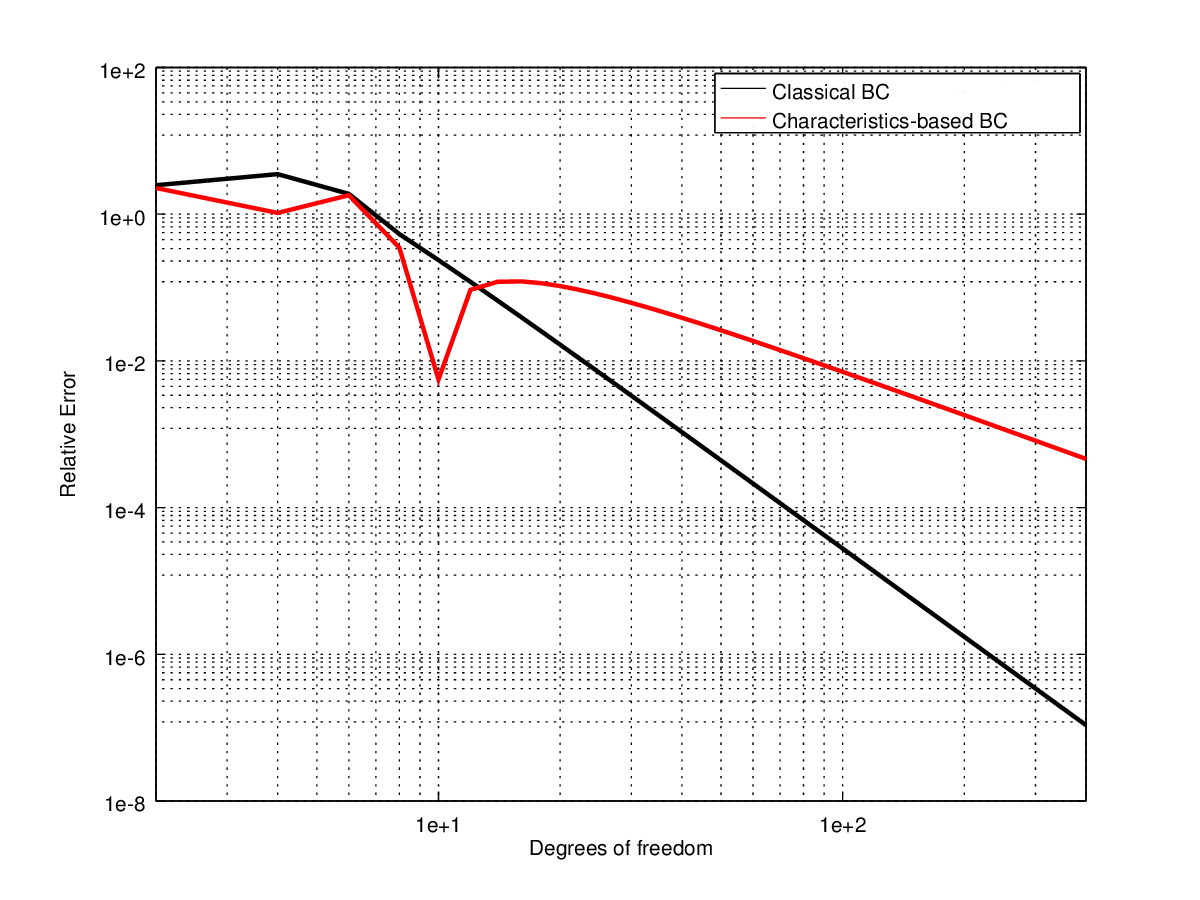
\includegraphics[width=10cm]{part3/figs/convergence.png}
	\caption{\label{fig:conv_DGMlike_quad}Erreur commise par les deux méthodes (ajout du coefficient de réflexion aux
	inconnues et caractéristiques) en fonction du nombre d'éléments utilisé. L'étude est réalisée uniquement pour des
	éléments quadratiques. Il faut noter que l'utilisation des caractériques donne de moins bons résultats dans ce cas.}
\end{figure}
